\documentclass{beamer}
\usetheme{Boadilla}

%typical packages
\usepackage{tikz,amsfonts,amsmath,pgfplots}

%typical tikz stuff
\tikzstyle{vertex}=[circle, draw, inner sep=0pt, minimum size=6pt,fill=white]
\newcommand{\vertex}{\node[vertex]}


\title{The Title of My Talk}
\subtitle{the Subtitle, if needed}
\author{my name}
\institute{University of Alaska Fairbanks}
\date{\today}

\begin{document}

 %TITLE PAGE
 \begin{frame}
\titlepage
\end{frame}

%Second Page
\begin{frame}

The document class (that very top line) is \fbox{beamer}. Go online and you'll find lots of help and alternative formatting.

\begin{center}

Each slide begins with \fbox{ $\backslash$begin\{frame\} } 
\vfill
and
\vfill
Ends with \fbox{ $\backslash$end\{frame\} } 

\end{center}

\end{frame}

%Third Page
\begin{frame}
\frametitle{Title of this page}
\vfill
\textcolor{red}{I can change the text color the same way.}
\begin{itemize}
	\item lists 
	\vfill
	\begin{itemize}
		\item work the same way
		\item really
		\vfill
	\end{itemize}
	\item So does mathematical formatting
	\vfill
	\begin{itemize}
		\item like $y=f(x)$
		\item and $\displaystyle{\int_0^1 e^x \: dx}$
		\vfill
	\end{itemize}
\end{itemize}
\end{frame}

% Third page
\begin{frame}
\frametitle{Tikz works too}
Steal a pic from HW 7:\\

\begin{center}
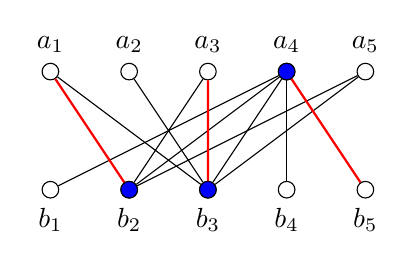
\begin{tikzpicture}
\foreach \i in {1,2,...,5}{
	\vertex (a\i) at (\i,1) [label=above:$a_{\i}$]{};
	\vertex (b\i) at (\i,-.5) [label=below:$b_{\i}$]{};
	}
\draw (b2) -- (a1) -- (b3) (a2)--(b3) (a3)--(b2) (b2) -- (a5) -- (b3);
\foreach \i in {1,2,...,5}{\draw (a4) -- (b\i);}
%%Red edges
\draw[thick, red] (b2)--(a1)(a3)--(b3)(a4)--(b5);
%blue vertices
\node[circle, draw, inner sep=0pt, minimum size=6pt,fill=blue] at (2,-.5){};
\node[circle, draw, inner sep=0pt, minimum size=6pt,fill=blue] at (3,-.5){};
\node[circle, draw, inner sep=0pt, minimum size=6pt,fill=blue] at (4,1){};
\end{tikzpicture}
\end{center}
\end{frame}

\end{document}

%Linearization:routine
\begin{frame}
\frametitle{Differential: Sample Routine Problems}
\begin{center}
\fbox{Find the \textcolor{blue}{differential} of $y=2x+\cos(x)$.}
\end{center}
\vspace{3in}
\end{frame}

%Linearization:routine
\begin{frame}
\frametitle{Differential: Sample Routine Problems}

\textbf{Example:} Find the \textcolor{blue}{differential} of $y=2x+\cos(x)$ and evaluate $dy$ when at $x=0$ and $dx=0.1$

\vspace{3in}
\end{frame}

%routine problems
\begin{frame}
\frametitle{Differential: Sample Routine Problem}
\vfill
\begin{center}\fbox{YOU WORK:}\end{center}
\vfill
Webassign \S 3.10 \#3,4,5
\vfill
\end{frame}

%differential: Interpretation
\begin{frame}
\frametitle{Differential: Interpretation}

We found
\begin{center} the differential of $y=2x+\cos x$ \end{center}
was
\begin{center} $dy=(2-\sin x) dx$ \end{center}
and when $x=0$ and $dx=0.1$
\begin{center} $dy=0.2$ \end{center}

\vspace{2in}
\end{frame}

\begin{frame}
\frametitle{Typical Book Example}
The edge of a cube is measured to be 20 cm with a possible error of $0.2$ cm. Use differential to estimate the maximum possible error in the calculation of the volume of the cube.\\
\vspace{2in}

YOU WORK: WebAssign \S 3.10 \#6; Written \S 3.10 \#34
\end{frame}


%%%%%%END%%%%%%%
\end{document}

\begin{frame}
\frametitle{}
\end{frame}

%where to find things
\begin{frame}
Where to find things:
	\begin{itemize}
	\item the course webpage: \textcolor{blue}{https://uaf-math251.github.io/}
	\item Blackboard: \textcolor{blue}{classes.alaska.edu}
	\end{itemize}
\end{frame}

%syllabus
\begin{frame}
the Syllabus
	\begin{itemize}
	\item Read it. (for all of your classes)
	\item Contacting by email.
	\item Grading rubric.
	\item An important calculation:
	
	\begin{center} If $100(0.1) + x(0.9)\geq 70,$ then 
	$x \geq 66.6$ \end{center}
	\item Midterms and Proficiency re-takes are given in the evening. 
	\item Resources
	\end{itemize}
\end{frame}

%resources
\begin{frame}
	Resources
	\begin{itemize}
	\item class 
	\item office hours
	\item Math Lab \& one-on-one tutoring
	\item old materials (worksheets, quizzes, proficiencies, midterms, finals) on Calculus I webpage
	\item old videos (on Blackboard)
	\item homework solutions (on Blackboard)
	\end{itemize}
\end{frame}

%class vs recitation
\begin{frame}
Typical Week\\
\begin{center}
\begin{tabular}{lllll}
Mon&Tue&Wed&Thurs&Fri \\
\hline
lecture&recitation&lecture&lecture&lecture\\
\hline
Jill/Ed&Dakota&Jill/Ed&Jill/Ed&Jill/Ed\\
\hline
new& review +&new&new&new\\
material&quiz&material&material&material\\
\hline
WRH due&&&&\\
\end{tabular}
\end{center}
\end{frame}

%Week 1 versus the rest of the semester
\begin{frame}
Week 1 is different
	\begin{itemize}
	\item No written homework.
	\item No WebAssign homework.
	\item No written quiz in Recitation (Tue 01/14 \& 01/21)
	\end{itemize}
\end{frame}

\begin{frame}
Week 1 is different....instead
	\begin{itemize}
	\item today: Log in to the CALCULUS I cohort of ALEKS PPL
	\item Take an Initial Assessment in ALEKS PPL (extra credit if completed by Wed 01/15)
	\item Homework 0: 10 hours in Learning Mode OR reach 90\% of ALEKS pie.
	\item Take a \emph{proctored} ALEKS PPL placement test on Tuesday Jan 21.
	\end{itemize}
\end{frame}

\begin{frame}
Week 1 is different
\begin{center}
\begin{tabular}{llllll}
week&Mon&Tue&Wed&Thurs&Fri \\
\hline \hline
1&01/13&01/14&01/15&01/16&01/17\\
& today&graphs&trig&exponentials&logarithms\\
&&&&&\\
&&&Aleks pretest&&sign-up\\
\hline \hline
2&01/20&01/21&01/22&01/23&01/24\\
& no class&proctored& start&&\\
&&ALEKS PPL&Calculus&&\\
\end{tabular}
\end{center}
\end{frame}

%Tip of the Week
\begin{frame}
Week One Matters\\
\vfill
How you spend your time this week has a significant and measurable impact on your likelihood of success in this class.
\vfill
\end{frame}

\begin{frame}
Week One Matters\\
\vfill
\begin{itemize}
\item Students who miss class in the first week pass at much lower rates than those who attend every class in the first week.
\item Students who complete all early assignments at 70\% or better pass at much higher rates than those who do not.
\item Higher \textit{proctored} ALEKS PPL scores correlate with higher passing rates.
\end{itemize}
\vfill
\end{frame}

\end{document}

\begin{frame}
\frametitle{Course Components}
\begin{itemize}
\item WebAssign
	\begin{itemize}
	\item online homework
	\item due periodically during the week
	\end{itemize}
\item Written Homework
	\begin{itemize}
	\item \emph{usually} due on Monday
	\item due at the beginning of class
	\item consists of problems from your textbook
	\end{itemize}
\item Quizzes: every Tuesday in Recitation
\item Test-like assessments
	\begin{itemize}
	\item two Proficiencies
	\item two Midterms
	\item one cumulative Final Exam
	\end{itemize}
\end{itemize}
\end{frame}

\begin{frame}
\frametitle{How do I keep track of assignments in this course?}
\begin{enumerate}
\item Attend class all 5 days every week.
\item Go to the course webpage: \\
\begin{center}{\large{\textbf{https://uaf-math251.github.io/}}} \end{center}
\begin{itemize}
	\item schedule
	\item syllabus
	\item homework assignments
	\item directions for starting WebAssign
	\item old quizzes, midterms, finals with complete solutions
	\end{itemize}
\item Go to Blackboard
	\begin{itemize}
	\item grades
	\item announcements
	\item old videos organized by textbook section
	\end{itemize}
\end{enumerate}
\end{frame}

\begin{frame}
\vfill
\begin{center}
\Large{Go to webpage + Blackboard.}
\end{center}
\vfill
\end{frame}

\begin{frame}
\vfill
\begin{center}
\Large{The most important thing to know.}
\end{center}
\vfill
\end{frame}

\begin{frame}
\frametitle{The most important thing to know.}
\includegraphics[scale=.4]{Early_Indicator_Grade_2.pdf}
\end{frame}
\end{document}
